\subsection{Integration by Parts (Reversing the Product Rule)}
When a $u$-substitution won't work because the integrand is the product of two functions that are not related by a derivative, integration by parts may be able to help us.
Starting from the product rule\footnote{This justification isn't completely rigorous because you can't always treat differentials like fractions, but the overall result is correct.},
\begin{align*}
	\dd{}{x}{(uv)} &= u\dd{v}{x} + v\dd{u}{x} \\
	\int{\dd{}{x}{(uv)}\d{x}} &= \int{u\dd{v}{x}\d{x}} + \int{v\dd{u}{x}\d{x}} \\
	\int{\d{(uv)}} &= \int{u\d{v}} + \int{v\d{u}} \\
	uv &= \int{u\d{v}} + \int{v\d{u}} \\
	\int{u\d{v}} &= uv - \int{v\d{u}}.
\end{align*}

Essentially, if we are integrating a function that is a product of something we can differentiate ($u$) and something we can integrate ($\d{v}$), then we can do integration by parts.
\begin{example}
	Solve the following indefinite integral:
	\begin{equation*}
		\int{x\sin{x}\d{x}}.
	\end{equation*}
\end{example}
\begin{answer}
	Since $x$ and $\sin{x}$ don't have any parts that are related by a derivative, a $u$-substitution wouldn't be helpful.
	However, we know how to differentiate $x$ and integrate $\sin{x}$, so integration by parts is a good strategy to try.
	\begin{align*}
		u = x &\text{ and } \d{u} = \d{x} \\
		\d{v} = \sin{x}\d{x} &\text{ and } v =\footnotemark -\cos{x} \\
		\int{x\sin{x}\d{x}} &= -x\cos{x} - \int{-\cos{x}\d{x}} \\
		&= -x\cos{x} + \sin{x} + C.
	\end{align*}
\end{answer}
\footnotetext{We don't include the $+C$ when integrating $\d{v}$. We'll still include one at the end.}

\subsubsection{LIPET (How to choose $u$)}
The tricky part of integration by parts is choosing what should be $u$ and what should be $\d{v}$.
If in the previous example we had instead chosen $u=\sin{x}$, we would have gotten that $\int{x\sin{x}\d{x}} = \frac{x^2}{2}-\int{\frac{x^2}{2}\cos{x}\d{x}}$, which although true, doesn't give us an easier function to integrate.
Generally, we want to choose $u$ such that $\d{u}$ is a ``simplier'' function to integrate.
This can mean a lower-degree polynomial, or getting rid of functions like $\ln{x}$ and replacing them with polynomials.
You can remember the acronym \textbf{LIPET} as a guide to help you.
\begin{itemize}[align=left, leftmargin=0.66in]
	\item[\textbf{L}ogarithms]
	\item[\textbf{I}nverse Trig Functions]
	\item[\textbf{P}olynomials]
	\item[\textbf{E}xponentials]
	\item[\textbf{T}rig Functions]
\end{itemize}

\begin{example}
	Solve the following indefinite integral:
	\begin{equation*}
		\int{x^3\ln{x}\d{x}}.
	\end{equation*}
\end{example}
\begin{answer}
	Following LIPET, we select $u = \ln{x}$.
	\begin{align*}
		u = \ln{x} &\text{ and } \d{u} = \frac{\d{x}}{x} \\
		\d{v} = x^3\d{x} &\text{ and } v = x^4/4 \\
		\int{x^3\ln{x}\d{x}} &= \frac{x^4\ln{x}}{4} - \int{\frac{x^3}{4}\d{x}} \\
		&= \frac{x^4\ln{x}}{4} - \frac{x^4}{16} + C.
	\end{align*}
\end{answer}


Sometimes, we might have to do integration by parts multiple times.
It might seem like integration by parts is leading us in circles, but this can actually be a good thing, allowing us to solve the integral if we're observant.
\begin{example}
	Solve the following indefinite integral:
	\begin{equation*}
		\int{e^{-x}\cos{x}\d{x}}.
	\end{equation*}
\end{example}
\begin{answer}
	Following LIPET, $u=e^{-x}$.
	\begin{align*}
		u = e^{-x} &\text{ and } \d{u} = -e^{-x}\d{x} \\
		\d{v} = \cos{x}\d{x} &\text{ and } v = \sin{x} \\
		\int{e^{-x}\cos{x}\d{x}} &= e^{-x}\sin{x} + \int{e^{-x}\sin{x}\d{x}}.
	\end{align*}
	
	Following LIPET, $u = e^{-x}$ again.
	\begin{align*}
		u = e^{-x} &\text{ and } \d{u} = -e^{-x}\d{x} \\
		\d{v} = \sin{x}\d{x} &\text{ and } v = -\cos{x} \\
		e^{-x}\sin{x} + \int{e^{-x}\cos{x}\d{x}} &= e^{-x}\sin{x} - e^{-x}\cos{x} - \int{e^{-x}\cos{x}\d{x}}
	\end{align*}
	
	It might seem like we've hit a dead end, since we're back trying to integrate the exact same function we started with.
	However, if we rearrange our equations a little bit, we'll see that we're actually really close to a solution.
	\begin{align*}
		\int{e^{-x}\cos{x}\d{x}} &= e^{-x}\sin{x} - e^{-x}\cos{x} - \int{e^{-x}\cos{x}\d{x}} \\
		2\int{e^{-x}\cos{x}\d{x}} &=\footnotemark\hspace{5pt} e^{-x}\sin{x} - e^{-x}\cos{x} + C \\
		\int{e^{-x}\cos{x}\d{x}} &= \frac{e^{-x}\sin{x} - e^{-x}\cos{x}}{2} + C.
	\end{align*}
\end{answer}
\footnotetext{We need to remember to include a $+C$. Usually it would come from completely solving an integral, but here we just did some rearranging.}

\subsubsection{Inverse Trig Functions}
We can use tabular integration to integrate the inverse trig functions.
We'll also end up applying two different strategies: Integration by parts and $u$-substitution to solve one integral.
\begin{align*}
	u = \arcsin{x} &\text{ and } \d{u} = \frac{1}{\sqrt{1-x^2}} \\
	\d{v} = \d{x} &\text{ and } v = x \\
	\int{\arcsin{x}\d{x}} &= x\arcsin{x} - \int{\frac{x}{\sqrt{1-x^2}}\d{x}} \\
	u = 1-x^2 &\text{ and } x\d{x} = \frac{-1}{2}\d{u} \text{ (this is a different $u$ than before)} \\
	&= x\arcsin{x} + \frac{1}{2}\int{\frac{\d{u}}{\sqrt{u}}} \\
	&= x\arcsin{x} + \frac{1}{2}\left(\frac{\sqrt{u}}{1/2}\right) + C \\
	&= x\arcsin{x} + \sqrt{u} + C \\
	&= x\arcsin{x} + \sqrt{1-x^2} + C.
\end{align*}

We can do the exact same thing to find the integral of $\arccos{x}$.
\begin{equation*}
	\int{\arccos{x}\d{x}} = x\arccos{x} - \sqrt{1-x^2} + C.
\end{equation*}


The integration by parts into $u$-substitution idea even works for $\arctan{x}$.
\begin{align*}
	u = \arctan{x} &\text{ and } \d{u} = \frac{1}{1+x^2} \\
	\d{v} = \d{x} &\text{ and } v = x \\
	\int{\arctan{x}\d{x}} &= x\arctan{x} - \int{\frac{x}{1+x^2}\d{x}} \\
	u = 1+x^2 &\text{ and } x\d{x} = \frac{1}{2}\d{u} \text{ (this is a different $u$ than before)} \\
	&= x\arctan{x} - \frac{1}{2}\int{\frac{\d{u}}{u}} \\
	&= x\arctan{x} - \frac{1}{2}\ln{\abs{u}} + C \\
	&= x\arctan{x} - \frac{1}{2}\ln{\abs{1+x^2}} + C.
\end{align*}

We can do the same thing to find the integral of $\arccot{x}$.
\begin{equation*}
	\int{\arccot{x}\d{x}} = x\arccot{x} + \frac{1}{2}\ln{\abs{1+x^2}} + C.
\end{equation*}


The integrals of $\arcsec{x}$ and $\arccsc{x}$ involve a special type of function you probably haven't seen before, $\text{arccosh}{x}$.
However, if you're familiar with this function and it's derivative, you can still apply integration by parts to find their antiderivatives.
\begin{align*}
	\int{\arcsec{x}\d{x}} &= x\arcsec{x} - \text{arccosh}{x} + C \\
	\int{\arccsc{x}\d{x}} &= x\arccsc{x} + \text{arccosh}{x} + C.
\end{align*}

\subsubsection{Tabular Integration}
If we're trying to integrate a function like $x^4e^{-x}$ using integration by parts, we quickly realize that we'll need to perform integration by parts 4 times, choosing the same value for $\d{v}$ every time.
Since this would be rather tedious and repetitive, we can extract the essential elements of integration by parts into a table and perform integration by parts many times without needing to repeat ourselves.


In integration by parts, we essentially choose one function ($u$) to continually differentiate and another ($\d{v}$) to continually integrate.
We then alternate signs with each iteration of integration by parts, due to negative signs canceling each other out.
So, in our table, we'll have three columns, one where we'll continually differentiate a function, usually until its a constant, a column to keep track of the sign, and a final column that we'll continually integrate.
Then, all we'll have to do is multiply across columns and sum across rows to get our result from repeated integration by parts.

\begin{example}
	Solve the following indefinite integral:
	\begin{equation*}
		\int{x^4e^{-x}\d{x}}.
	\end{equation*}
\end{example}
\begin{answer}
	Following LIPET, $x^4$ is our function to differentiate and $e^{-x}$ is our function to integrate.
	Setting up our table,
	\begin{figure}[H]
		\label{tabular}
		\centering
		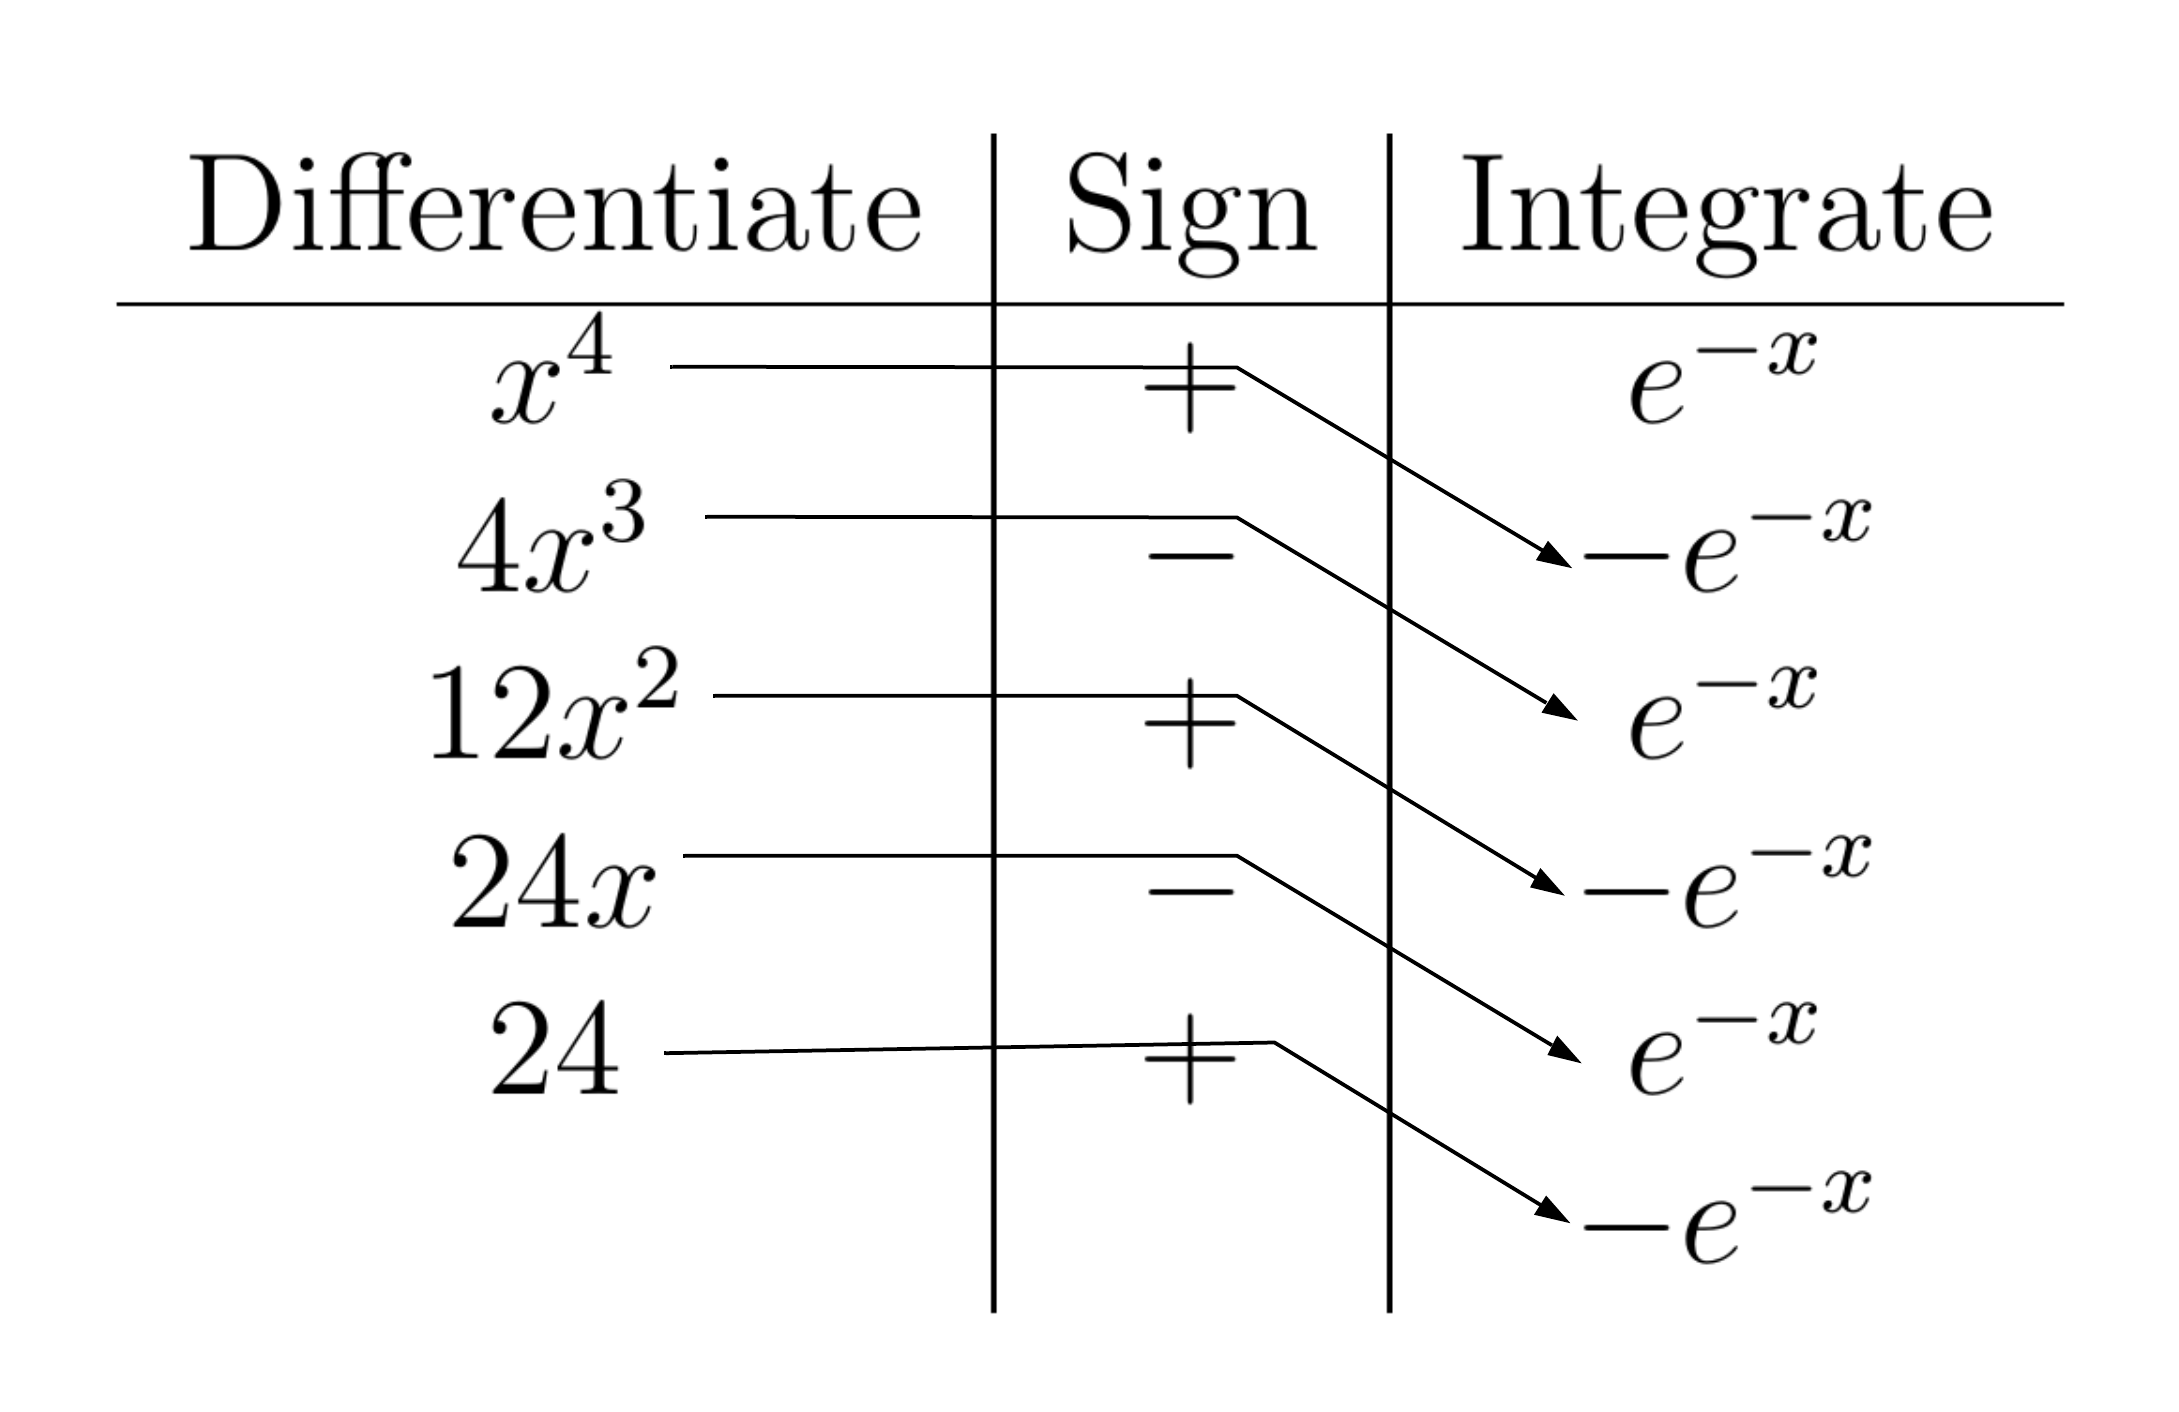
\includegraphics[width = 0.5\textwidth]{./integrals/integration_by_parts/tabular.png}
	\end{figure}
	Multiplying across each arrow and summing,
	\begin{align*}
		\int{x^4e^{-x}\d{x}} &= x^4\left(-e^{-x}\right) + 4x^3(-1)e^{-x} + 12x^2\left(-e^{-x}\right) + 24x(-1)e^{-x} + 24\left(-e^{-x}\right) + C \\
		&= -x^4e^{-x} - 4x^3e^{-x} - 12x^2e^{-x} - 24xe^{-x} - 24e^{-x} + C \\
		&= -e^{-x}\left(x^4 + 4x^3 + 12x^2 + 24x + 24\right) + C.
	\end{align*}
\end{answer}